\begin{figure*}
\centering
\begin{subfigure}[b]{0.33\textwidth}
\centering
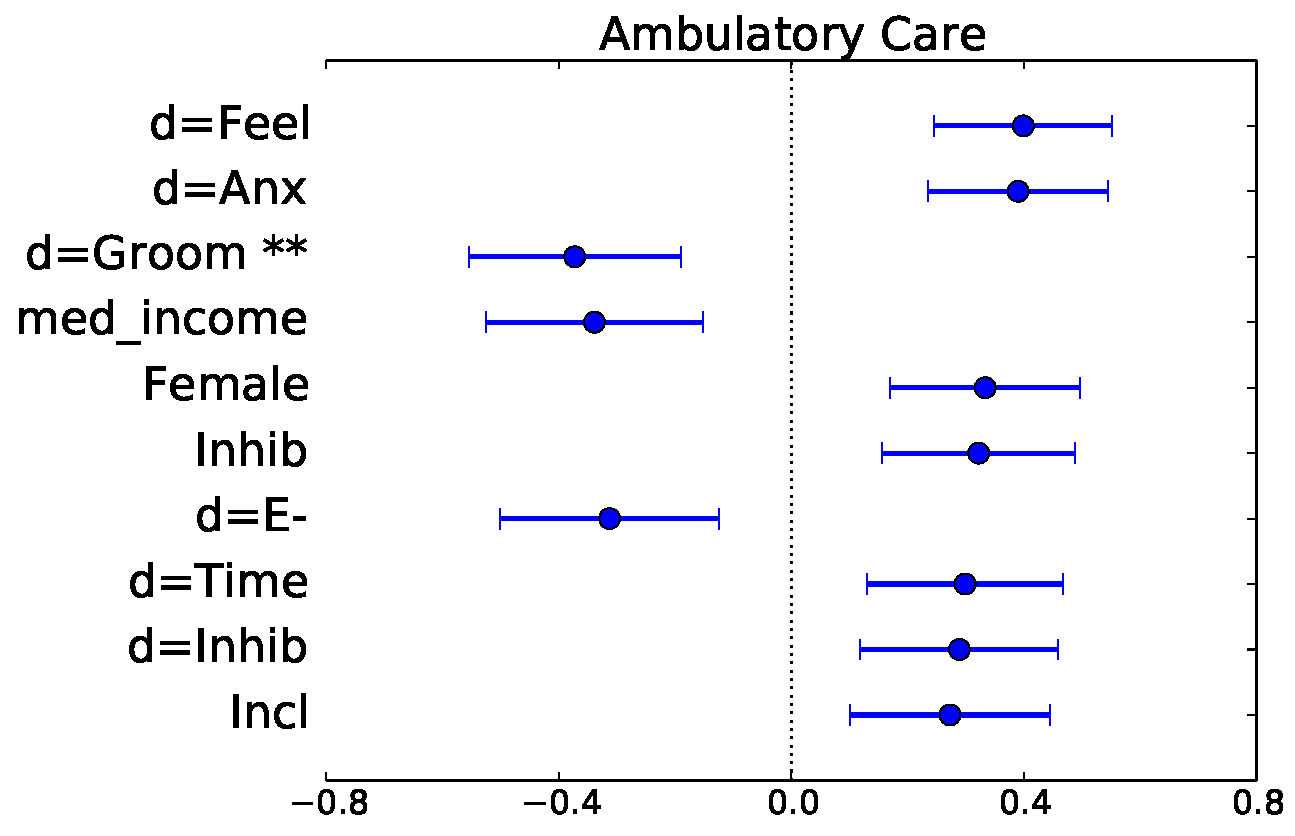
\includegraphics[width=\columnwidth,height=.6\columnwidth]{figs/ambulatorycaresensitiveconditions}
\label{fig.ambulatorycaresensitiveconditions}
\end{subfigure}
\begin{subfigure}[b]{0.33\textwidth}
\centering
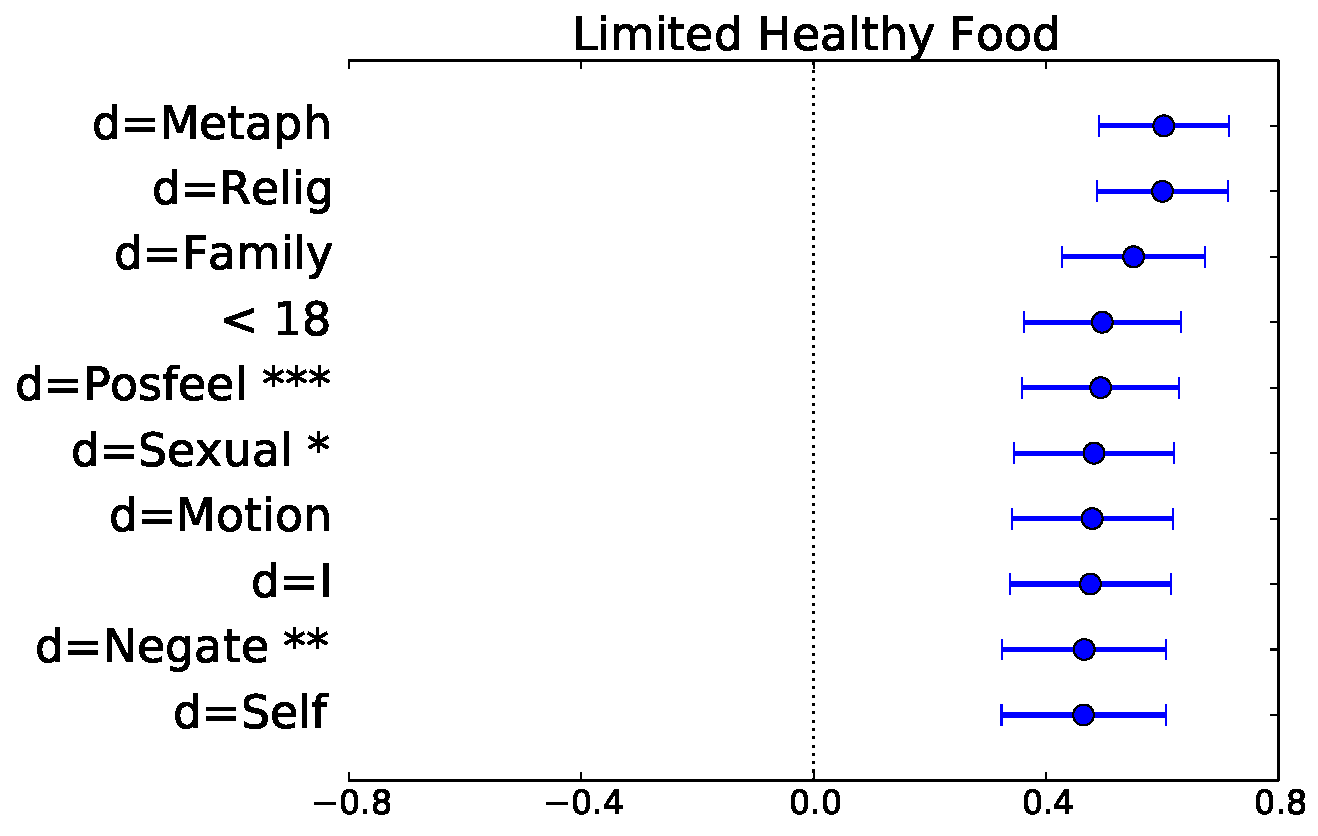
\includegraphics[width=\columnwidth,height=.6\columnwidth]{figs/limitedaccesstohealthyfoods}
\label{fig.limitedaccesstohealthyfoods}
\end{subfigure}
\begin{subfigure}[b]{0.33\textwidth}
\centering
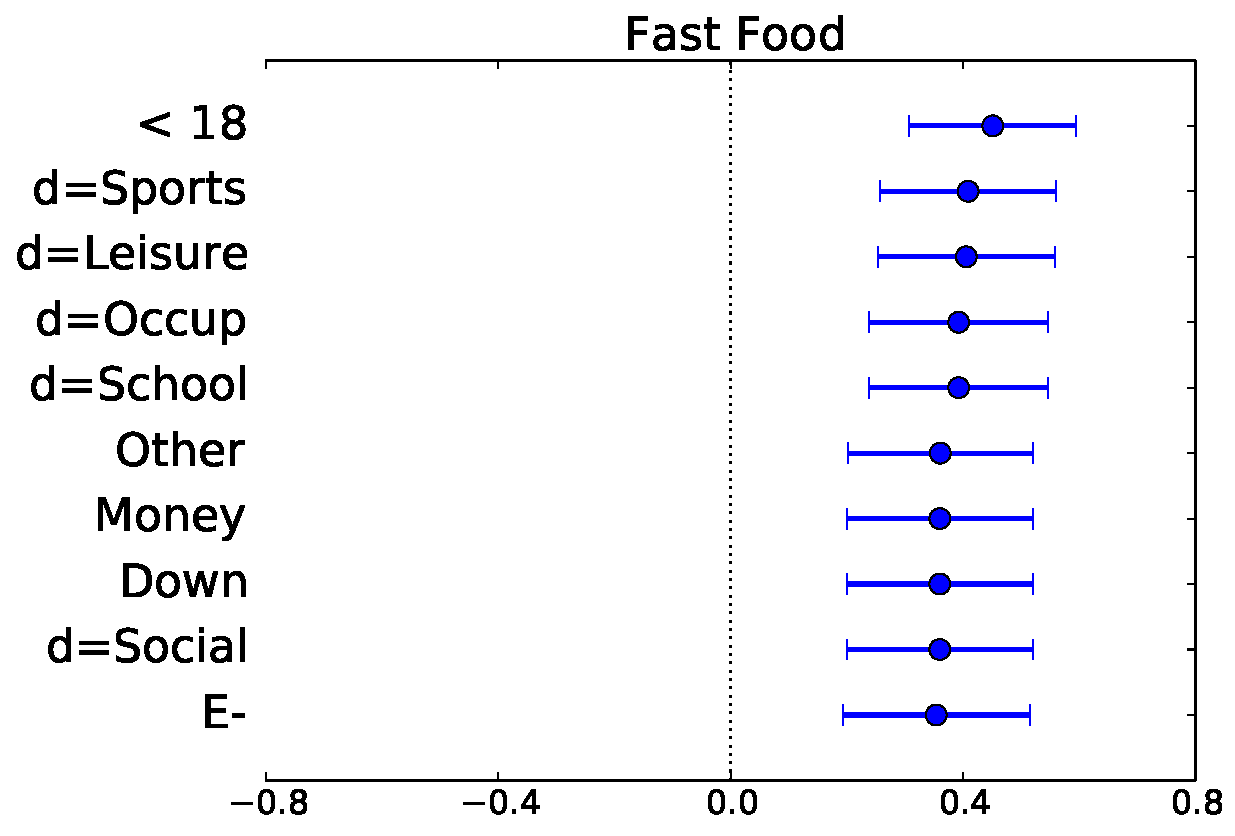
\includegraphics[width=\columnwidth,height=.6\columnwidth]{figs/fastfoods}
\label{fig.fastfoods}
\end{subfigure}
\begin{subfigure}[b]{0.33\textwidth}
\centering
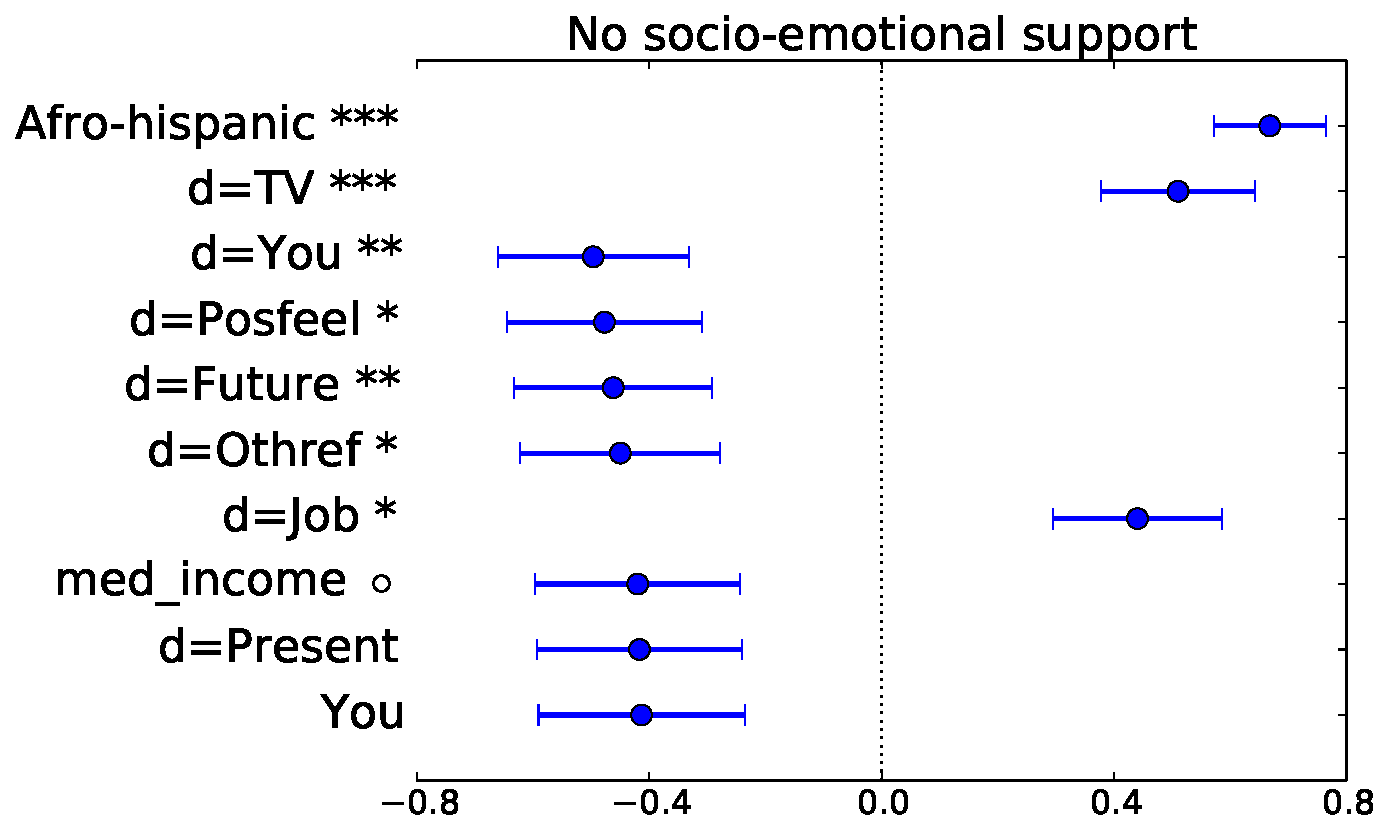
\includegraphics[width=\columnwidth,height=.6\columnwidth]{figs/nosocialemotionalsupport}
\label{fig.nosocialemotionalsupport}
\end{subfigure}
\begin{subfigure}[b]{0.33\textwidth}
\centering
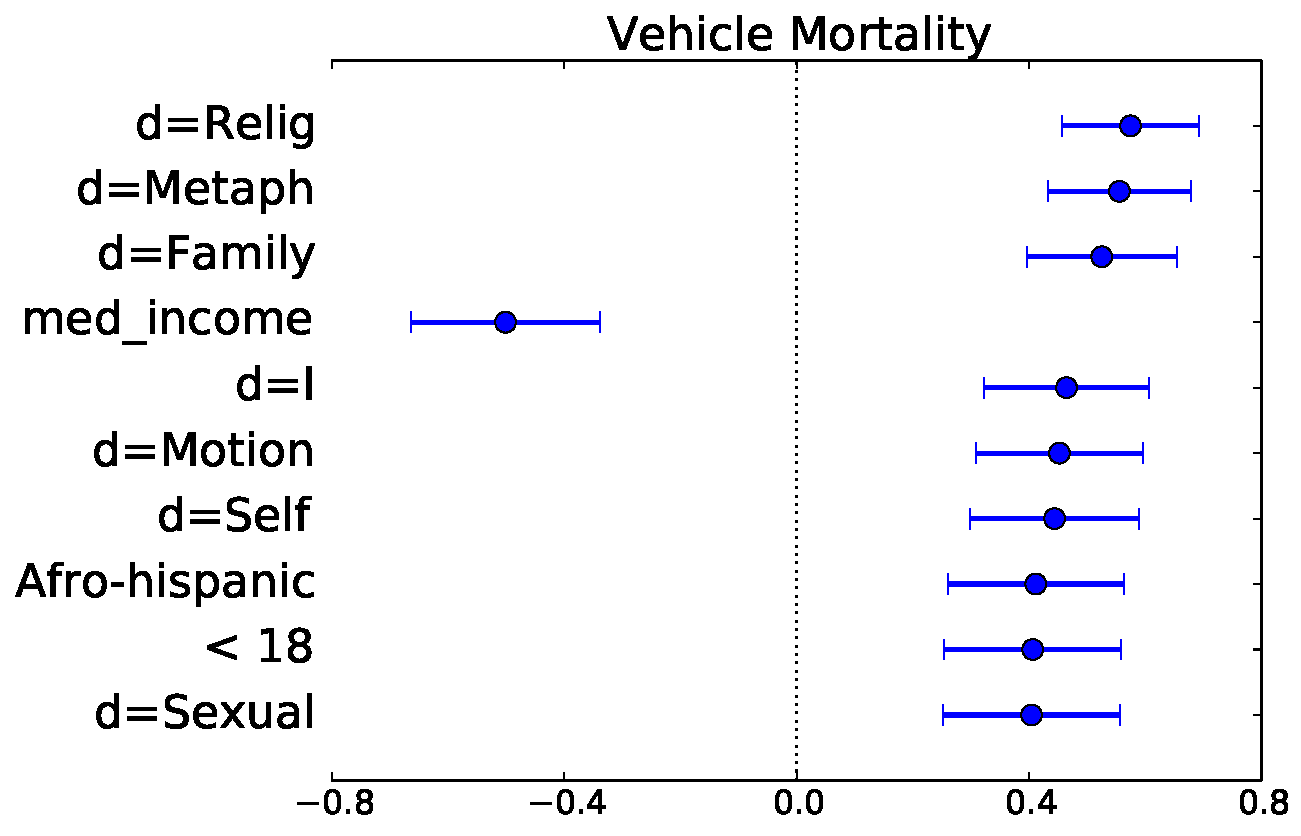
\includegraphics[width=\columnwidth,height=.6\columnwidth]{figs/mvmortalityrate}
\label{fig.mvmortalityrate}
\end{subfigure}
\begin{subfigure}[b]{0.33\textwidth}
\centering
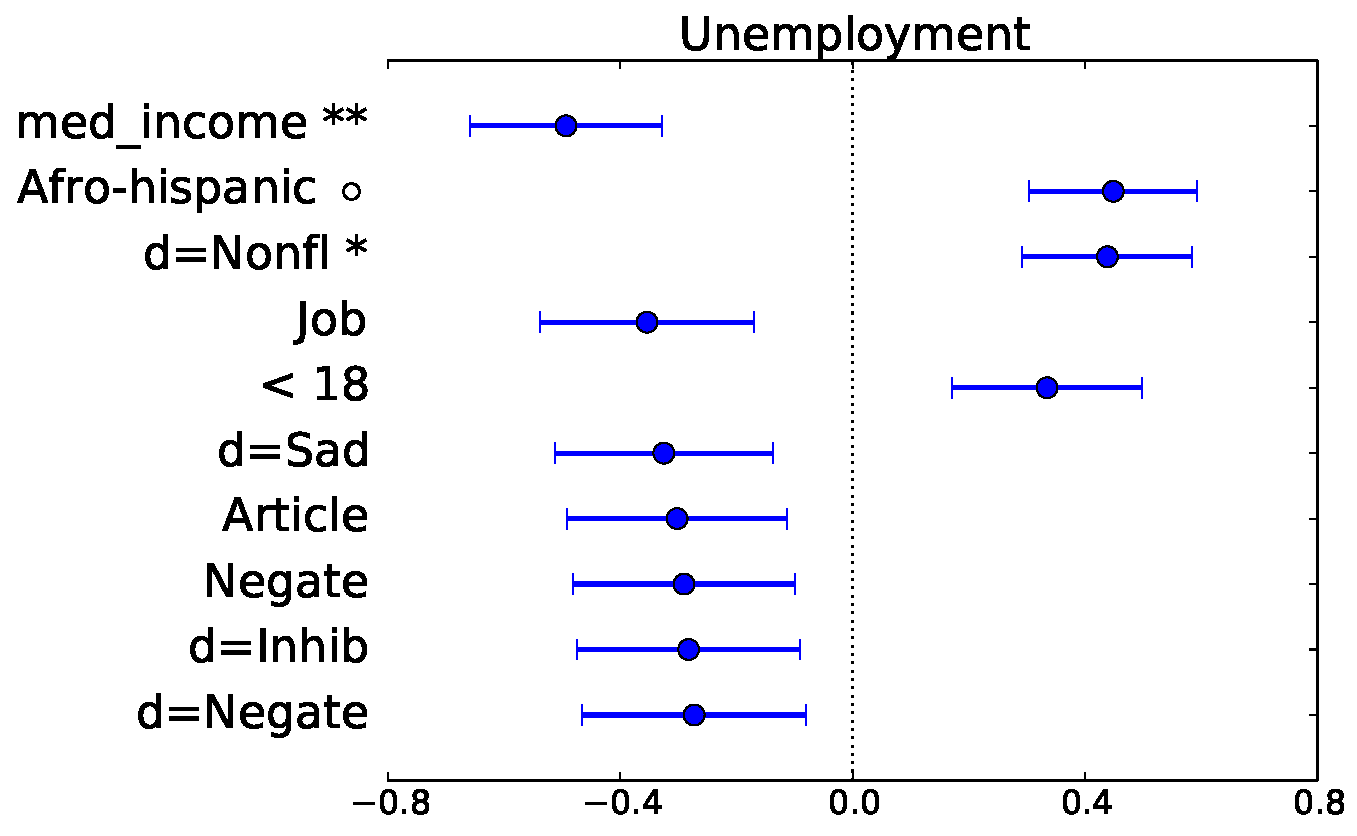
\includegraphics[width=\columnwidth,height=.6\columnwidth]{figs/unemployed}
\label{fig.unemployed}
\end{subfigure}
\begin{subfigure}[b]{0.33\textwidth}
\centering
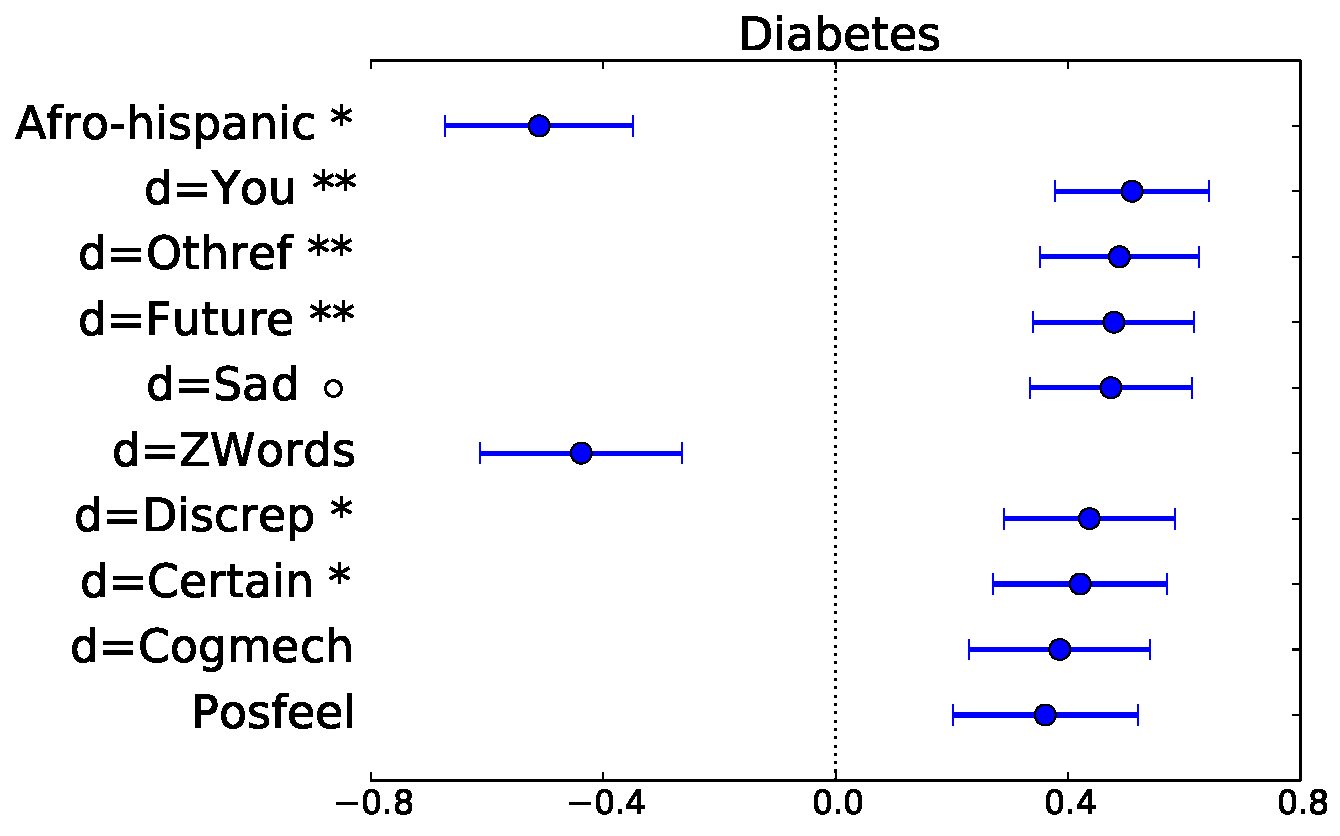
\includegraphics[width=\columnwidth,height=.6\columnwidth]{figs/hba1c}
\label{fig.hba1c}
\end{subfigure}
\begin{subfigure}[b]{0.33\textwidth}
\centering
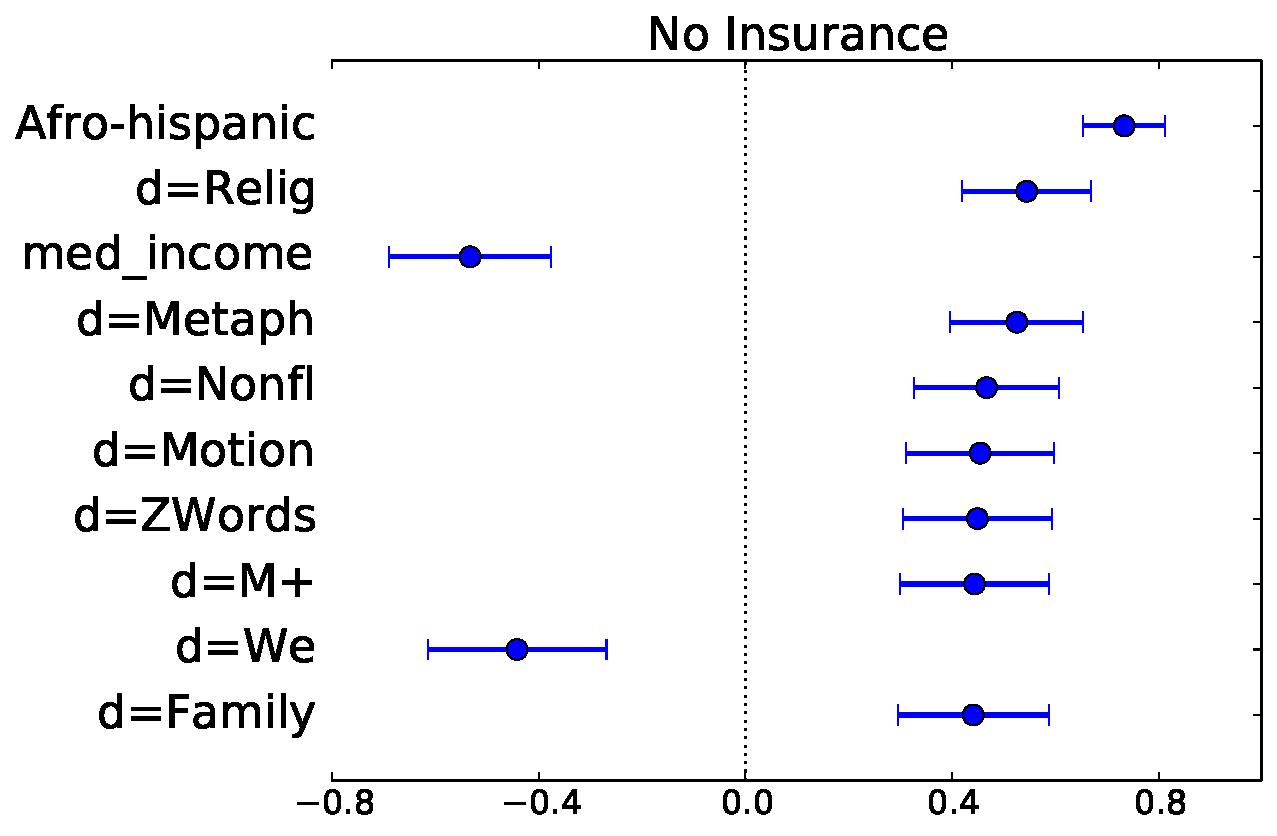
\includegraphics[width=\columnwidth,height=.6\columnwidth]{figs/uninsured}
\label{fig.uninsured}
\end{subfigure}
\begin{subfigure}[b]{0.33\textwidth}
\centering
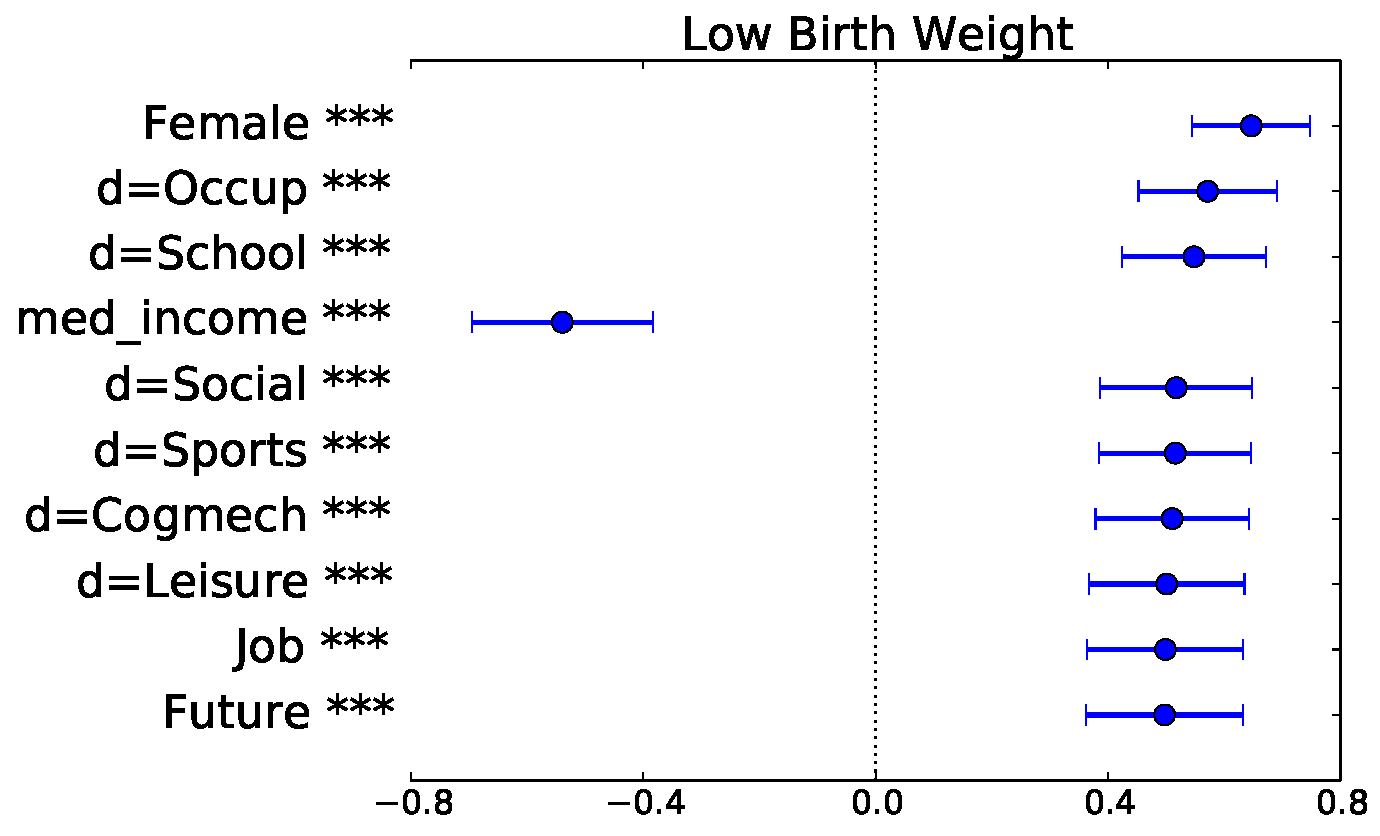
\includegraphics[width=\columnwidth,height=.6\columnwidth]{figs/lowbirthweight}
\label{fig.lowbirthweight}
\end{subfigure}
\begin{subfigure}[b]{0.33\textwidth}
\centering
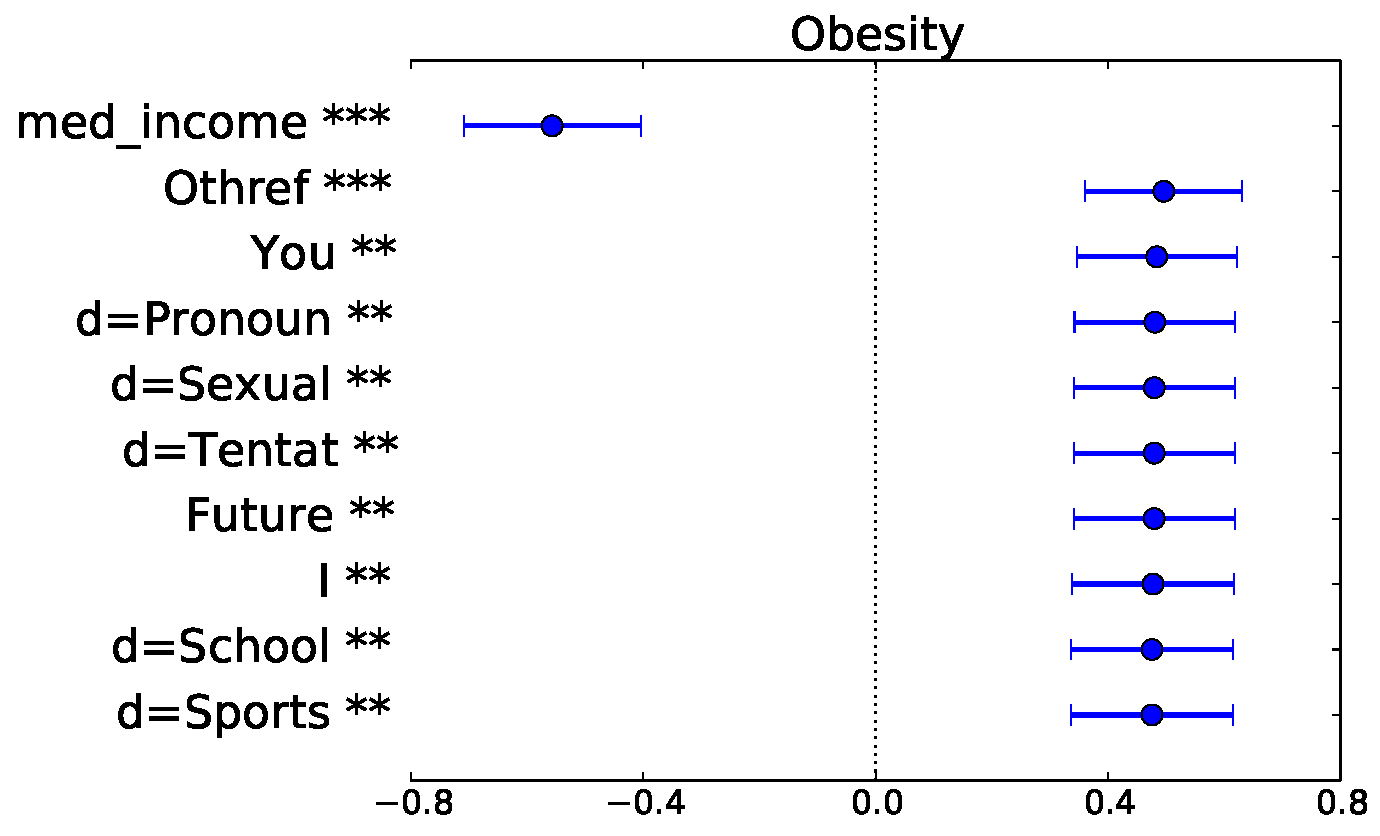
\includegraphics[width=\columnwidth,height=.6\columnwidth]{figs/obese}
\label{fig.obese}
\end{subfigure}
\begin{subfigure}[b]{0.33\textwidth}
\centering
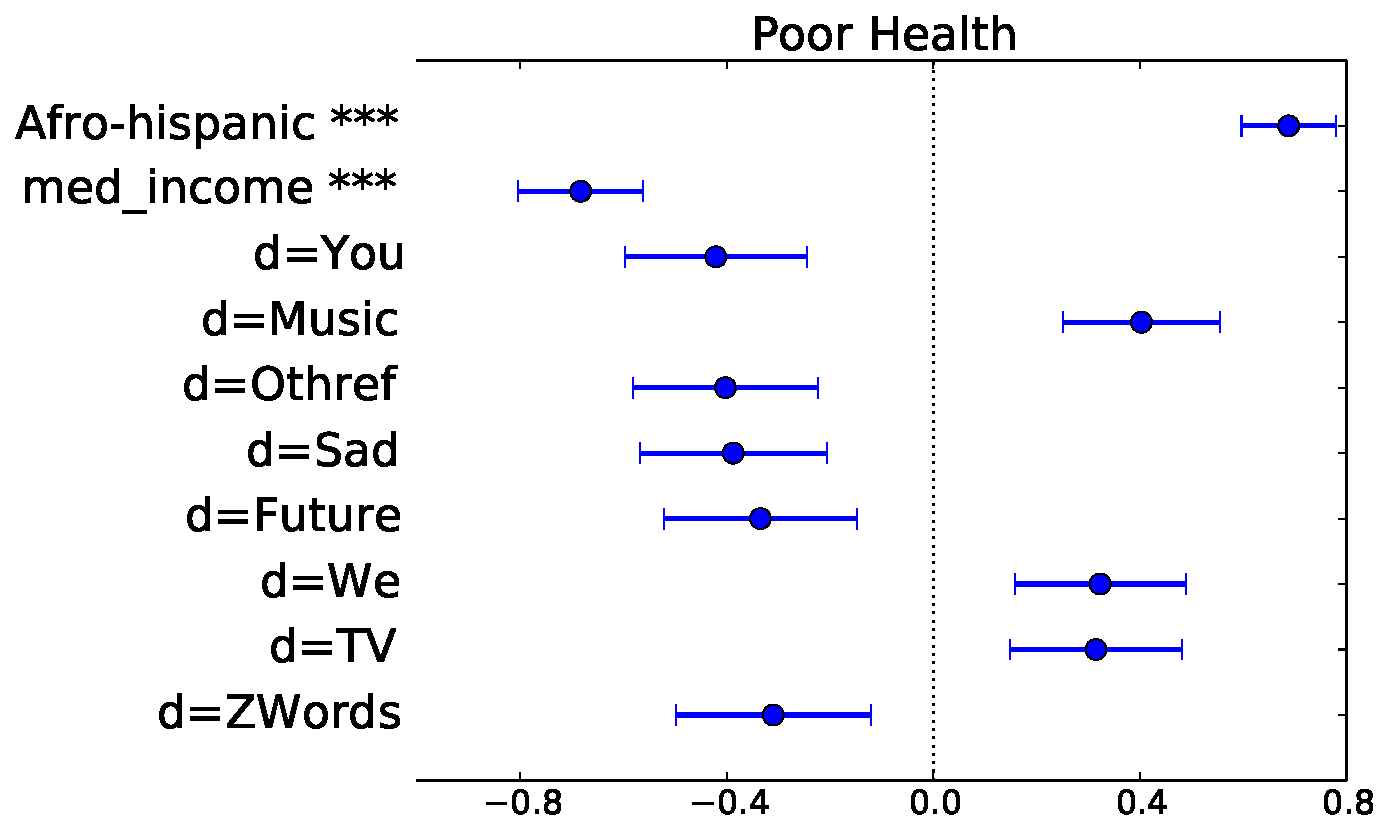
\includegraphics[width=\columnwidth,height=.6\columnwidth]{figs/fairpoorhealth}
\label{fig.fairpoorhealth}
\end{subfigure}
\begin{subfigure}[b]{0.33\textwidth}
\centering
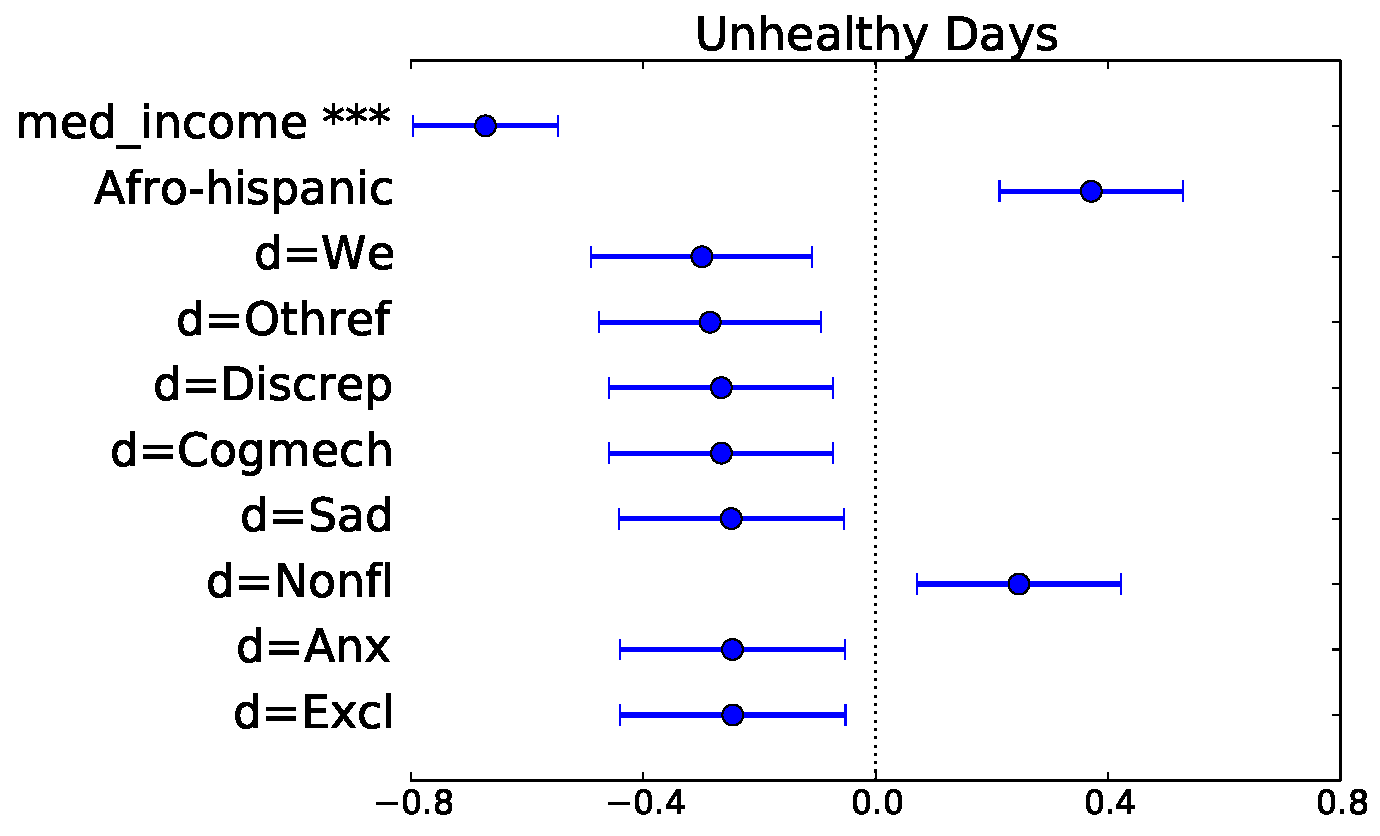
\includegraphics[width=\columnwidth,height=.6\columnwidth]{figs/physicallyunhealthydays}
\label{fig.physicallyunhealthydays}
\end{subfigure}
\caption{For the top 12 outcomes in Table \ref{tab.outcomes}, we plot the 10 variables with the highest correlation (error bars denote the 95\% confidence interval.) Statistical significance is indicated by $\circ = 0.1$, $\ast = 0.05$, $\ast\ast = 0.01$, $\ast\ast\ast = 0.001$ (degress of freedom = 98). The thresholds have been Bonferroni-corrected using the total number of variables (160) times the number of outcomes (27). The prefix {\sl d=} denotes lexical categories from the description field of a user's Twitter profile. Otherwise, the categories are derived from the tweet text. For comparison, the control variables are also included. \label{fig.words} }
 \end{figure*}